\chapter{\label{c:waveguides}Measurement of transverse-to-longitudinal phase coupling in a waveguide mirror}
\chaptermark{Waveguide transverse-to-longitudinal phase coupling}

\emph{The following chapter has been adapted from \emph{Upper limit to the transverse to longitudinal motion coupling of a waveguide mirror \cite{Leavey2015}}, published in \emph{Classical and Quantum Gravity} in 2015. The article was entirely written by the author and is suitable for inclusion, expanded as appropriate, within this thesis. The results and conclusions presented are identical.}

\section{Thermal noise in advanced detectors}
At their most sensitive frequencies, the second generation detectors are expected to be limited by Brownian thermal noise arising from the reflective coatings on the detectors' test masses \cite{Levin1998, Nakagawa2002, Harry2002, Crooks2002}. In order to help mitigate this limitation beyond the next generation of detectors, efforts are under way to develop mirror coatings with lower thermal noise \cite{Flaminio2010, Bassiri2013}.

In the case of Advanced LIGO, each end test mass (\gls{ETM}) consists of a substrate with \num{19} pairs of sub-wavelength coatings which produce a transmission of \SI{5}{ppm} for \SI{1064}{\nano\meter} light with very little loss \cite{Dannenberg2009}, with each coating layer contributing to the overall thermal noise \cite{Harry2002, Crooks2002}. The approach taken by Levin to calculate the thermal noise of mirrors \cite{Levin1998} shows that mechanical loss at the front surface of a mirror contributes more to the Brownian noise level than loss from an equivalent volume in the substrate. Additionally, typical coating materials tend to exhibit mechanical loss orders of magnitude higher than typical substrate materials \cite{Harry2002, Crooks2002}. For these reasons particular attention is being given to the reduction of coating thermal noise to improve the sensitivity of future detectors.

One strategy, to be applied for example in \KAGRA{} \cite{Sakakibara2014}, is to cool the mirrors to cryogenic temperatures. While this can potentially reduce the thermal noise of the mirrors \cite{Uchiyama2012}, the application of cryogenic mirrors requires new infrastructure, different choices of mirror substrate and coating materials and poses the challenge of heat extraction from the mirror without spoiling its seismic isolation and thermal noise performance. Efforts in the application of cryogenics are also under way to identify suitable substrate and coating materials for \ETLF{}, the low frequency interferometer as part of the proposed \ET{} \cite{Punturo2010, Martin2010, Hild2011, Abernathy2011}, and the proposal for a cryogenic upgrade to \LIGO{}, Voyager \cite{aligoinst2015}.

\section{Waveguide and grating mirrors}
Apart from using different coating materials \cite{Granata2013, Cole2013} or different beam shapes \cite{Mours2006, DAmbrosio2004, Bondarescu2006} such as with LG33 modes \cite{Sorazu2013}, another potential approach is to utilise waveguide mirrors (\glspl{WGM}) \cite{Brueckner2008, Brueckner2009, Brueckner2010, Friedrich2011}. These mirrors can possess high reflectivity at a wavelength determined by their structure. In contrast to conventional dielectric mirrors, mirrors possessing waveguide coatings can exhibit high reflectivity without requiring multiple stacks \cite{Bunkowski2006}. A waveguide coating instead presents incident light with a periodic grating structure of high refractive index material $n_H$ on top of a substrate with low refractive index $n_L$ (see Figure\,\ref{fig:waveguide-reflection}). Light is forced into a single reflective diffraction order, the \nth{0}. In transmission, only the \nth{0} and \nth{1} diffraction orders are allowed as long as the condition in Equation~\ref{eq:grating-equation} for the grating period, $p$, and the light's wavelength in vacuum, $\lambda$, is fulfilled \cite{Brueckner2008}. The light diffracted into the \nth{1} order undergoes total internal reflection at the substrate boundary where it excites resonant waveguide modes. With suitable parameters the light at the waveguide boundary to the incident beam will contain a \SI{180}{\degree} phase shift with respect to the \nth{0} order transmitted light, causing destructive interference such that most of the incident light is reflected \cite{Sharon1997}.

\begin{equation}
  \frac{\lambda}{n_{H}} < p < \frac{\lambda}{n_{L}}
  \label{eq:grating-equation}
\end{equation}

\begin{figure}
  \centering
  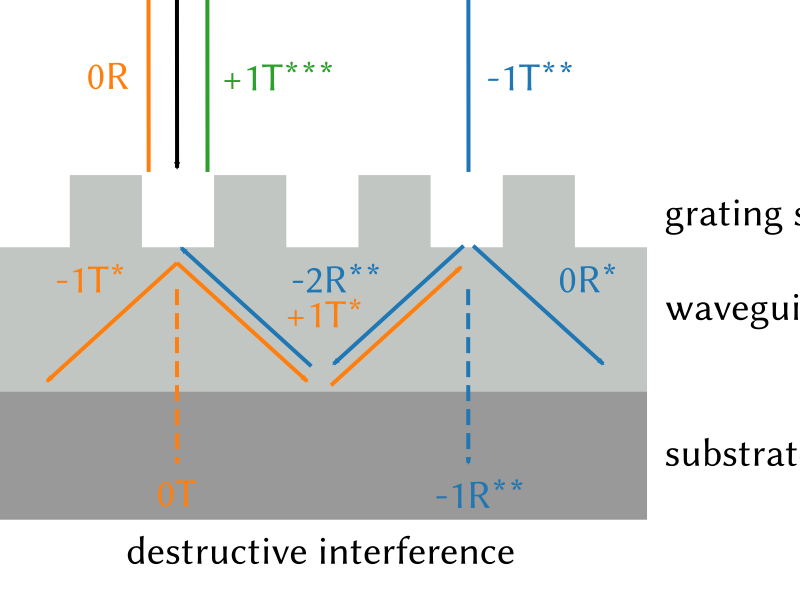
\includegraphics[width=0.6\textwidth]{graphics/generated/from-svg/30-waveguide-reflection.pdf}
  \caption[Propagation of light within a waveguide mirror]{\label{fig:waveguide-reflection}Propagation of light within a waveguide mirror (a reproduction of Fig.\,1 from \cite{Brown2013}). The grating and waveguide layers have refractive index $n_H$, and sit atop a substrate of refractive index $n_L$. The incident light (black) diffracts into the first orders $\pm 1$ (orange). At the substrate the light reflects and at the grating the light either interferes with the incident light to produce reflection or reflects back into the waveguide (blue). The numbers next to the arrows represent the diffraction order, $T$ represents transmission through the grating, $R$ represents reflection from the grating and each asterisk represents a single diffraction. The grating parameters can be tuned such that the phase difference at the front (waveguide) surface produces high reflection. In realisations of waveguide mirrors such as this, a thin etch-stop layer is placed between the grating and waveguide layers to assist fabrication \cite{Friedrich2011}.}
\end{figure}

We have shown in \cite{Heinert2013} that a suitably optimised \gls{WGM} can provide a reduction in coating thermal noise amplitude of a factor of 10 at cryogenic temperature compared to the \gls{ETM} employed in Advanced LIGO. Figure\,\ref{fig:coating-vs-grating-noise} shows Brownian thermal noise modelled for different numbers of bilayers (following \cite{Harry2002}) for the Advanced LIGO \gls{ETM} alongside the grating thermal noise result from Heinert \etal{}. For each additional bilayer in the dielectric stack, the mirror's transmissivity decreases but its Brownian thermal noise increases. The grating, however, requires only a change in grating parameters to produce a specific transmissivity, and this does not have a strong dependence on Brownian thermal noise.

\begin{figure}
  \centering
  \input{graphics/generated/from-python/30-coating-vs-grating-noise.pgf}
  \caption[Brownian thermal noise in an Advanced LIGO style end test mass at room temperature versus that of a waveguide mirror at cryogenic temperature, as a function of transmissivity]{\label{fig:coating-vs-grating-noise}Reproduction of the results from Heinert \etal{} \cite{Heinert2013} showing Brownian thermal noise in an Advanced LIGO style \gls{ETM} at room temperature versus that of a \gls{WGM} at cryogenic temperature, as a function of transmissivity. The markers in the coating curve represent the number of quarter-wavelength bilayers forming the dielectric stack. Each additional bilayer in the coating stack produces lower overall transmissivity, but also increases Brownian thermal noise. The grating's Brownian thermal noise contribution is independent of transmissivity. The transmissivity of Advanced LIGO's \gls{ETM} is shown as a vertical, dashed line.}
\end{figure}

\subsection{Transverse to longitudinal coupling in grating mirrors}

Previous efforts to demonstrate grating structures as alternatives to dielectric mirrors have identified phase noise in the light reflected from the grating not otherwise present in dielectric mirrors \cite{Wise2005, Freise2007}. This effect arises from transverse motion of grating mirrors with respect to the incident light. Incident light at angle $\alpha$ is reflected into the m\textsuperscript{th} diffraction order, exiting at angle $\beta_m$ (see Figure\,\ref{fig:grating-propagation}). The change in path length $\delta l_L$ between the reflected and incident light is then
\begin{equation}
  \delta l_L = \zeta_a + \zeta_b = \delta y
  \left( \sin{\alpha} + \sin{\beta_m} \right),
\end{equation}
where $\zeta_a$ and $\zeta_b$ represent the relative optical path length of each depicted ray.
The phase modulation induced in the reflected light by periodic, transverse motion of the \gls{WGM} is proportional to the period with a \SI{90}{\degree} phase lead over the transverse motion \cite{Barr2011}. The frequency noise added to the reflected light can be enough to mitigate the improvement in coating thermal noise, as witnessed in a study of \nth{2} order Littrow gratings \cite{Barr2011}, where the level of coupling between longitudinal and transverse motion was found to be 1:100. Although \glspl{WGM} also possess gratings, the resonant waveguide structure can be tuned to remove this effect as shown in simulations by Brown \emph{et al.} \cite{Brown2013}.

\begin{figure}
  \centering
  \includegraphics[width=0.5\textwidth]{graphics/generated/from-svg/30-grating-propagation.pdf}
  \caption[Optical path length changes $\zeta_a$ and $\zeta_b$ due to transverse motion of a Littrow grating]{\label{fig:grating-propagation}Optical path length changes $\zeta_a$ and $\zeta_b$ due to transverse motion of a Littrow grating, based on Figure\,4 of \cite{Freise2007}. Incident light diffracted into a different order undergoes a path length change $\delta l_L = \zeta_a + \zeta_b$.}
\end{figure}

There are two mechanisms by which grating mirrors can couple transverse motion into longitudinal phase changes (see Figure\,\ref{fig:waveguide-scanning}). The first is through transverse motion of the grating, which can in principle be minimised with appropriate suspension design. The second mechanism is the coupling of changes in the opposite cavity mirror's alignment into the spot position on the grating mirror. This effect is of particular importance to gravitational wave interferometers, where longer arm lengths can increase its detrimental impact. The latter mechanism is the primary focus of this work.

\begin{figure}
  \centering
  \includegraphics[width=0.5\columnwidth]{graphics/generated/from-svg/30-waveguide-scanning.pdf}
  \caption[Two ways in which light can be scanned across the surface of a waveguide mirror]{\label{fig:waveguide-scanning}Two ways in which light can be scanned across the surface of the \gls{WGM}. The left panel shows the effect of \gls{WGM} motion with respect to a static beam, while the right panel shows the effect of light beam motion (due to rotation of the cavity mirror opposite the \gls{WGM}) with respect to a static \gls{WGM}. In the latter picture, the cavity's eigenmode is translated transversely to the optical axis as one mirror is rotated.}
\end{figure}

In order to quantify its transverse coupling, a \gls{WGM} was produced in collaboration with Friedrich-Schiller University Jena, Germany; see Table \ref{tab:waveguide-parameters} for its properties. It was designed for light of wavelength \SI{1064}{\nano\meter}, and consists of an etched grating structure on top of a waveguide layer, both tantala (\ce{Ta_2O_5}), on a silica substrate. This chapter details an experiment carried out to measure its transverse coupling level.

\begin{table}
  \centering
  \begin{tabular}{|l|l|}
    \hline
    \textbf{Parameter}    & \textbf{Value}            \\ \hline
    Materials             & \ce{SiO_2}, \ce{Ta_2O_5}, \\
			  & \ce{Al_2O_3}              \\ \hline
    Design $\lambda$      & \SI{1064}{\nano\meter}    \\ \hline
    Grating depth         & \SI{390}{\nano\meter}     \\ \hline
    Waveguide depth       & \SI{80}{\nano\meter}      \\ \hline
    Etch stop depth       & \SI{20}{\nano\meter}      \\ \hline
    Grating period        & \SI{688}{\nano\meter}     \\ \hline
    Fill factor           & 0.38                      \\ \hline
    Reflectivity          & 96\%                      \\ \hline
  \end{tabular}
  \caption[Design parameters of the waveguide mirror for the experiment to measure transverse to longitudinal coupling]{\label{tab:waveguide-parameters}Design parameters of the \gls{WGM} produced by Friedrich-Schiller Jena for the experiment to measure transverse to longitudinal coupling. It is similar to the one used in \cite{Friedrich2011}, with increased reflective surface area.}
\end{table}

\section{Experiment}

The fabricated \gls{WGM} was used as the input coupler for a \FP{} cavity, held on resonance using the Pound-Drever-Hall (\gls{PDH}) technique \cite{Drever1983}. The error signal provided by the \gls{PDH} technique represents changes in cavity length, and this can be fed back to the laser's frequency via a frequency stabilisation servo. This technique is described in more detail in Section\,\ref{sec:pdh}.

\subsection{Effect of waveguide mirror rotation on cavity length}
\label{sec:lengthsignals}

A non-zero \gls{WGM} transverse to longitudinal coupling, $\omega_1$, produces a phase shift on the reflected light. This manifests itself as an effective change in cavity length, $\delta l_W$, as the laser light is scanned across its grooves by the rotation of the \gls{ETM}:
\begin{equation}
  \label{eq:wgm-length-change}
  \delta l_W = \theta \kappa \omega_1,
\end{equation}
where $\theta$ is the \gls{ETM}'s (small) rotation angle and $\kappa$ is the cavity's coefficient of \gls{ETM} rotation to transverse \gls{WGM} spot displacement.

Additional cavity length changes from mirror rotation are created by two geometrical effects as shown in Figure\,\ref{fig:mirror-longitudinal-effect}. The first effect, $\delta l_s$, is due to the position of the beam with respect to the centre of the mirror's surface. For a rotation $\theta$, a beam offset from the centre of the mirror by a displacement $y$ will receive a change in (longitudinal) path length of:
\begin{equation}
  \label{eq:offset-effect}
  \delta l_s = y \tan{\theta} \approx y \theta,
\end{equation}
for small angles. The second effect, $\delta l_d$, is due to the depth $d$ of the mirror, proportional to the rotation angle $\theta$. The position of the centre of the mirror with respect to the zero rotation case, $y_d$, is then:
\begin{equation}
  y_d = \frac{d}{2} \tan{\frac{\theta}{2}} \approx \frac{d}{4} \theta,
\end{equation}
and the change in path length this causes is:
\begin{equation}
  \delta l_d = y_d \tan{\theta} \approx \frac{d}{4} \theta^2.
\end{equation}
The total longitudinal effect $\delta l_E$ caused by the rotation of the \gls{ETM} is therefore:
\begin{equation}
  \label{eq:etm-length-change}
  \delta l_E = \delta l_s + \delta l_d \approx y \theta + \frac{d}{4} \theta^2,
\end{equation}
and the total length signal from all mirror effects will then be:
\begin{equation}
  \label{eq:cavity-length-change}
  \delta l \left( \theta \right) = \delta l_W + \delta l_E \approx \theta \kappa \omega_1 + y \theta + \frac{d}{4} \theta^2.
\end{equation}

\begin{figure}
  \centering
  \includegraphics[width=0.5\columnwidth]{graphics/generated/from-svg/30-mirror-longitudinal-effect.pdf}
  \caption[Geometrical end test mass longitudinal coupling]{\label{fig:mirror-longitudinal-effect}Geometrical \gls{ETM} longitudinal coupling. For a given rotation $\theta$ and spot centre position offset $y$, the (longitudinal) position change in the surface of the mirror (show in blue) as seen by the reflected light is approximately $y \theta + \frac{d}{4} \theta^2$. The straight, solid red line in the figure shows this longitudinal change.}
\end{figure}

\subsection{Cavity length signals}
Considering the \gls{ETM}'s dimensions and mass, it is possible to calculate the cavity length change due to the two geometrical effects shown in Equation~\ref{eq:etm-length-change} for a given rotation. From the cavity length change it is then possible to infer the \gls{WGM}'s transverse to longitudinal coupling level using Equation~\ref{eq:cavity-length-change}. The phase effect associated with transverse to longitudinal coupling is expected to be independent of the average spot position, whereas there is a phase change about the \gls{ETM}'s centre of rotation. It is expected therefore that a spot position will exist, for a non-zero \gls{WGM} transverse coupling level, offset from the \gls{ETM}'s centre of rotation, for which there is a cavity error signal minimum. This effect arises as a result of the coherent cancellation of $\delta l_W$ and $\delta l_{E}$ (see Figure\,\ref{fig:coupling-contributions}). The spot position corresponding to the error signal minimum allows the \gls{WGM}'s transverse to longitudinal coupling level to be inferred.

Examples of \gls{WGM} coupling levels yielding cavity length changes smaller than (green), larger than (blue) and roughly equivalent to (orange) the \gls{ETM}'s effects are shown in Figure\,\ref{fig:coupling-contributions}. For cases where the \gls{WGM}'s coupling level yields a significant cavity length change with respect to that of the \gls{ETM}'s rotation, coherent cancellation creates a trough significantly offset from the \gls{ETM}'s centre of rotation.

\begin{figure}
  \centering
  \input{graphics/generated/from-python/30-individual-factors.pgf}
  \caption[Simulations of indicative cavity longitudinal error signals during end test mass rotation for different levels of waveguide mirror coupling]{\label{fig:coupling-contributions}Simulations of indicative cavity longitudinal error signals during \gls{ETM} rotation for different levels of \gls{WGM} coupling. The signals are functions of the transverse position of the reflected light relative to the \gls{ETM}'s centre of rotation, the angle of rotation, the mirror depth and the \gls{WGM}'s coupling level. The rotation to longitudinal coupling of the \gls{ETM} (black dashed line) combines with the transverse to longitudinal coupling of the \gls{WGM} (green, orange and blue dashed lines) to produce cavity length changes (green, orange and blue solid lines). In this example configuration, the \gls{ETM} rotation is \SI{1e-7}{\radian}, the \gls{ETM}'s depth is \SI{0.1}{\meter} and the corresponding \gls{WGM} coupling levels are 1:370 (blue), 1:3700 (orange) and 1:37000 (green).}
\end{figure}

% Coupling levels in fig:coupling-contributions
% rotation angle is 1e-7 rad (from plot_individual_factors script, an arbitrary choice, not the real level of rotation used in the experiment)
% rotation to sidemotion calibration from the experiment is 18.5119047619 metres / rad
%
% so sidemotion is 1851 nm
%
% red: longitudinal signal is 5e-9 m, so coupling is 1:370
% green: 5e-10 m, so 1:3702
% blue: 5e-11, so 1:37024

\subsection{Experiment infrastructure}
\label{sec:glasgow10m}

The \GLASGOWTENM{} facility provides a test bed in which the \gls{WGM}'s transverse to longitudinal coupling can be quantified. The prototype is housed in a Class 1000 clean room and consists of an input bench at atmospheric pressure and a vacuum envelope able to reach pressures of order \SI{e-3}{\pascal}. The envelope consists of nine \SI{1}{\meter} diameter steel tanks, each connected by steel tubes, arranged into two parallel arms of length \SI{10}{\meter}, with a shorter arm for input optics situated between them.

In the experiment, \SI{1064}{\nano\meter} laser light was passed through a single-mode fibre to provide spatial filtering, and an electro-optic modulator (\gls{EOM}) to impose \gls{RF} sidebands on the light required to produce an error signal with the \gls{PDH} technique. The light was then coupled into the vacuum system via a periscope. A control system senses the motion of the cavity with the \gls{RF} photodiode near Tank 1 and provides corrective actuation on the laser crystal's piezoelectric transducer (\gls{PZT}) and temperature via a frequency stabilisation servo and associated electronics (see Section\,\ref{sec:cavity-length-measurement}). This configuration is shown in Figure\,\ref{fig:prototype-setup}.

\begin{figure}
  \centering
  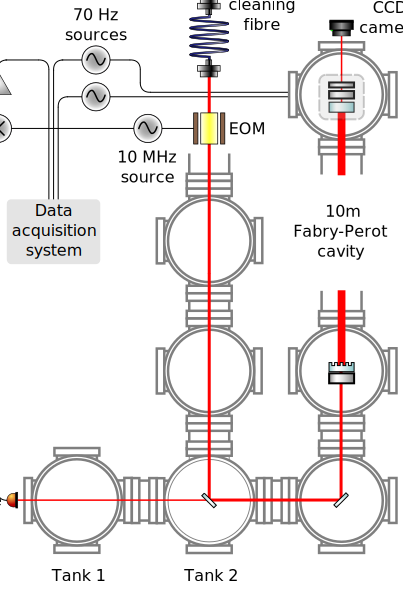
\includegraphics[width=\columnwidth]{graphics/generated/from-svg/30-waveguide-arm-in-prototype.pdf}
  \caption[Experimental setup for measurement of waveguide transverse to longitudinal coupling]{\label{fig:prototype-setup}The experimental setup in the prototype facility. The laser light is passed through input optics (not shown), a mode cleaning fibre and an \gls{EOM} before being coupled into the vacuum system via a periscope. It then travels to Tank 2 where it is reflected off a beam splitter and directed into one of the arms of the prototype by a steering mirror in Tank 3. The two mirrors in Tanks 4 and 5 form a \FP{} cavity. The cavity mirrors are suspended from triple stage suspensions, and the beam splitter and steering mirror are both suspended from double suspensions. \\
  \\The \gls{ETM} is rotated in yaw using the \SI{70}{\hertz} source. It is fed to a coil driver where it is coupled into Tank 5 via a vacuum feedthrough. Coil formers on the front edges of the reaction mass contain wound copper wire connected to the vacuum feedthrough. Magnets are attached to the back of the \gls{ETM}. The reaction mass is behind the \gls{ETM}, containing a hole in its centre to allow light to exit the vacuum tank where it can be viewed with the CCD camera. A larger version of the contents of Tank 5 can be viewed in the panel to the right of the figure. \\
  \\The cavity is held on resonance by the frequency stabilisation servo. This feeds back to the light's frequency via the laser crystal's temperature below \SI{12}{\hertz} and its PZT above \SI{12}{\hertz} up to a unity gain frequency of \SI{16}{\kilo\hertz} (see Section\,\ref{sec:cavity-control}).}
\end{figure}

Tanks 2 and 3 house a beam splitter and steering mirror, respectively, attached to double stage suspensions. In Tanks 4 and 5 were sets of two triple suspension chains based on the \GEO{} design \cite{Plissi2000}. A viewport present to the rear of Tank 5, and to the side of Tank 1, allowed for light to exit the vacuum envelope for the purposes of sensing and control.

The \gls{WGM} was attached to an aluminium block of mass \SI{2.7}{\kilo\gram} and suspended from Tank 4's cascaded (triple) pendulum, forming the cavity's \gls{ITM}. A silica test mass, also \SI{2.7}{\kilo\gram}, with a \SI{40}{ppm} transmission coating, was used as the \gls{ETM}, suspended from a similar triple pendulum in Tank 5. On the rear surface of the \gls{ETM} were three magnets for the purpose of actuation, the positions of which are shown in Figure\,\ref{fig:etm-rear}. With optimal alignment the mirrors formed an overcoupled cavity with finesse \num{155}.

\begin{figure}
  \centering
  \includegraphics[width=0.4\columnwidth]{graphics/generated/from-svg/30-etm-rear.pdf}
  \caption[Positions of the magnets on the rear surface of the end test mass used in the waveguide experiment]{\label{fig:etm-rear}The positions of the magnets on the rear surface of the \gls{ETM}. The designations used in this article are shown next to each magnet. The top magnet is positioned at the centre of yaw, near the top of the mass. The left and right magnets are positioned \SI{56.3}{\milli\meter} either side of the centre of yaw. Coils on the \gls{ETM}'s reaction mass (not shown) are positioned coaxially behind each magnet.}
\end{figure}

A three-stage reaction chain was placed behind the triple pendulum of the \gls{ETM} to provide voice coil actuation upon the magnets on the \gls{ETM}'s rear surface. The upper and intermediate stages were identical to those of the chain carrying the \gls{ETM}, however\textemdash for the purposes of another experiment, not reported here\textemdash the lower stage was split into two parts separately suspended from the intermediate stage. The part closer to the \gls{ETM} was a \SI{1.8}{\kilo\gram} aluminium block that carried the voice coils. The other part was a \SI{0.9}{\kilo\gram} aluminium block required to balance the suspension.

\begin{table}
  \centering
  \begin{tabular}{|l|l|}
    \hline
    \textbf{Parameter}        & \textbf{Description}	      \\ \hline
    Cavity input power      & Approx. \SI{150}{\milli\watt}   \\ \hline
    \gls{ETM} transmissivity      & $40$~ppm                  \\ \hline
    \gls{ETM} radius of curvature & \SI{15}{\meter}           \\ \hline
    \gls{ETM} spot size           & \SI{2.138}{\milli \meter} \\ \hline
    \gls{ITM} transmissivity      & \SI{4}{\%}                \\ \hline
    \gls{ITM} radius of curvature & $\infty$                  \\ \hline
    \gls{ITM} spot size           & \SI{1.554}{\milli \meter} \\ \hline
    Cavity length           & \SI{9.81}{\meter}               \\ \hline
    Cavity finesse          & \SI{155}{}                      \\ \hline
    Cavity g-factor         & \SI{0.347}{}                    \\ \hline
    Beam waist size         & \SI{1.554}{\milli \meter}       \\ \hline
    Beam waist position     & At \gls{ITM}                    \\ \hline
    Sideband frequency      & \SI{10}{\mega\hertz}            \\ \hline
  \end{tabular}
  \caption[Cavity parameters]{\label{tab:cavity-parameters}Cavity parameters.}
\end{table}

\subsection{\label{sec:cavity-length-measurement}Measuring cavity length changes}

An \gls{RF} photodetector was placed at the viewport on Tank 1, where it could view the light reflected from the cavity. By using the \gls{PDH} technique (see Section\,\ref{sec:pdh}), the signal from this photodetector provided an error signal for the cavity length. This signal was fed back to the laser via the frequency stabilisation servo to maintain cavity resonance. The servo's high frequency feedback signal\textemdash a voltage applied across the laser's \gls{PZT}\textemdash provided a means of calibrating cavity length changes at frequencies greater than \SI{12}{\hertz}. Using the \gls{PZT}'s actuator coefficient, \SI{1.35}{\mega\hertz \per \volt_{rms}}, the cavity length change $\delta l$ per error signal volt could be calculated to be \SI{133}{\nano\meter \per \volt_{peak}}.

\subsubsection{\label{sec:pdh}The Pound-Drever-Hall technique}
Several techniques exist to control cavity length fluctuations, the earliest of which was through the use of \emph{\gls{DC} locking}. This involves keeping the power on a photodetector constant by feeding back an error signal to either the laser's frequency or to actuators on the cavity mirrors. The error signal arises from a change in measured photodetector power from some set point. This set point is in the case of \gls{DC} locking necessarily away from the dark fringe, because at that point a cavity length increase or decrease results in an identical drop in power incident upon the photodetector and thus cannot be used as a discriminant for cavity length. Instead, the set point must be somewhere on the slope leading to or from the peak, where a length increase has opposite sign compared to a length decrease. As the set point is not situated at the operating point producing maximum cavity power build-up, and thus sensitivity, this technique has since been superseded by a range of techniques that result in superior performance. Dither locking \cite{White1965}, which uses a dither signal applied to a mirror to act as a local oscillator to the carrier from which an error signal can be derived, was used for the output mode cleaner of Enhanced LIGO \cite{Ward2008}. Another technique, tilt locking \cite{Shaddock1999}, uses the beat between the first and fundamental spacial modes of the carrier. We will however focus on a fourth technique, Pound-Drever-Hall (\gls{PDH}) \cite{Drever1983, Black2001}, which is particularly suited for \FP{} experiments requiring good sensitivity across a wide bandwidth.

As described in Appendix\,\ref{a:interferometry}, phase modulation cannot be detected by standard photodetector electronics. Although modulation due to the presence of phase sidebands leads to a change in light power, this change happens on time scales too short for a photodiode to register a change in its electronic signal: any stray capacitance in its material or transmission lines filters the phase modulation in the same way as a low pass filter, averaging the modulation to zero. Figure\,\ref{fig:cavity-tf}, however, shows that the phase of the error signal from a cavity detuned from resonance appears to be a good error signal: it is bipolar about the optimal operating point. The \gls{PDH} technique provides access to this phase information.

The key features of \gls{PDH} are highlighted below. More detailed descriptions can be found in, for example, \cite{Freise2010} and \cite{Black2001}. Mirror motion imparts phase modulation upon the carrier as shown in Section\,\ref{sec:signal-sidebands}. Restating Equation\,\ref{eq:field-phase-mod-expanded} we see that phase modulation upon the carrier produces upper and lower sidebands with frequencies $\omega_0 \pm \omega$, where $\omega$ represents the phase modulation frequency:
\begin{equation}
  \label{eq:field-phase-mod-expanded-30}
  E = E_0 \text{e}^{\text{i} \omega_0 t} \left( 1 - \frac{m^2}{4} + \text{i} \frac{m}{2} \left( \text{e}^{-\text{i} \omega t} + \text{e}^{\text{i} \omega t} \right) \right),
\end{equation}
assuming sub-wavelength motion.

Phase modulation can also be intentionally imparted upon the carrier through the use of an \gls{EOM}, as depicted in Figure\,\ref{fig:prototype-setup}. With the \gls{PDH} technique, the \gls{EOM} is placed in the path of the cavity's input light where it imparts strong phase modulation to the carrier at \gls{RF} frequencies. The choice of this frequency band is motivated by the availability of low cost and low noise electronics, the lack of \SI{1064}{\nano\meter} laser frequency noise, and the avoidance of the audio band where experiments in the field of ground-based gravitational wave interferometry typically desire high sensitivity. The \gls{RF} sidebands produced by the \gls{EOM} must be chosen to be greater than the cavity's \gls{FWHM} (see Section\,\ref{sec:cavity-fom}) to prevent them from entering the cavity. As the carrier light resonates within the cavity and reflects back towards the laser, any phase modulation imparted to the carrier by mirror motion beats with the \gls{RF} sidebands that do not enter the cavity, with the difference in phase showing up as signal sidebands upon the \gls{RF} sidebands. The signal sidebands can be recovered from the field through demodulation at the \gls{RF} frequency.

In a typical \gls{PDH} setup, a frequency generator is fed both to the \gls{EOM} and to a mixer connected to the output of an \gls{RF} photodetector placed in reflection of the cavity (see Figure\,\ref{fig:prototype-setup}). This ensures that the same frequency used to create the \gls{RF} sidebands is used to demodulate the superposition of fields reflecting from the cavity. Mixing the oscillator's signal with the reflected light is equivalent to multiplying the reflected field by a factor of $\sin{\omega t}$ or $\cos{\omega t}$, which yields a signal with frequency components proportional to the cavity motion at those frequencies. This signal is bipolar, with cavity mirror motion in one direction yielding a different sign to motion in the other direction. This \emph{error} signal can be fed back to the cavity's actuators to hold the cavity resonant.

\subsubsection{\label{sec:cavity-control}Cavity control}
The reflected light from the cavity was sensed with the \gls{RF} photodiode placed near Tank 1. This was mixed in order to demodulate the field and recover the cavity error signal, and this was coupled into an analogue servo containing filters designed to keep the \FP{} cavity on resonance. This analogue servo design resembles that of the servo presented in \cite{Macarthur2014}, and contains feedback paths to the laser's temperature and \gls{PZT}, able to correct the laser's frequency at low and high frequencies, respectively, thus providing a way to maintain the cavity resonance condition. Estimated open loop gains of both the temperature and \gls{PZT} feedback are shown in Figure\,\ref{fig:servo-tf}. The \gls{PZT} feedback is flat below \SI{30}{\hertz}, where the temperature feedback servo performs the majority of the actuation. Above this point, a slope proportional to $\frac{1}{f^3}$ removes feedback at higher frequencies to provide greater control bandwidth for corrections at low frequencies where it is most needed due to seismic noise (see Appendix\,\ref{sec:control-bandwidth}). A differentiator is present above \SI{3}{\kilo\hertz} to correct the phase of the feedback signal to allow it to cross below the unity gain point without creating unstable signals with equal magnitude but opposite sign to the measured motion, as discussed in Appendix\,\ref{sec:gain-phase-margin}. A copy of the feedback to the \gls{PZT} is sent to \gls{CDS} where a series of filters produce the temperature feedback signal. Gain is applied to the low frequency components to ensure the laser temperature's signal is strong where its response is strong. Additional resonant gain is applied at the suspension resonance frequency of \SI{0.6}{\hertz} to prevent it from ringing. One further filter is used to provide a stable crossover with the \gls{PZT} feedback at around \SI{12}{\hertz}. Above \SI{12}{\hertz} the response of the temperature feedback is greatly suppressed due to material's time constant. The unity gain point of the combined servo is around \SI{16}{\kilo\hertz}.

\begin{figure}
  \centering
  \input{graphics/generated/from-python/30-servo-tf.pgf}
  \caption[Waveguide cavity frequency stabilisation servo open loop gain]{\label{fig:servo-tf}Estimated open loop gain of the analogue servo used to feed the cavity error signal back to the laser's temperature and \gls{PZT}. The laser temperature actuator provides the majority of the feedback below \SI{12}{\hertz}, where it has a strong response. Its effect is significantly reduced above this point, where the time constant of the material becomes significant. The \gls{PZT} actuator provides actuation at higher frequencies, where it can provide smaller but faster corrections up to many tens of \SI{}{\kilo\hertz}. Various filters are required to produce stable temperature-to-\gls{PZT} crossover and unity gain points. The frequency used for measurements discussed later is shown as a dashed line.}
\end{figure}

\section{\label{sec:measurements}Measurements and analysis}

From the orientation of the \gls{WGM}'s gratings, it was expected that actuation of the \gls{ETM} in yaw, which would scan the cavity light across the \gls{WGM}'s surface transverse to the direction of its grooves, would exhibit \gls{WGM} transverse to longitudinal coupling if present.

\subsection{Voice coil balancing}
For the purposes of actuation upon the \gls{ETM}, two sinusoidal signals $V_L$ and $V_R$ (corresponding to the left and right voice coils on the \gls{ETM}'s reaction mass, respectively) were produced using separate, phase locked signal generators. A signal frequency of \SI{70}{\hertz} was chosen so as to be above the suspensions' pole frequencies, where the mirror's dynamics approximate that of a free mass, but low enough to provide an adequate \gls{RMS} test mass rotation. The signals $V_L$ and $V_R$, with suitable balancing (see below), could then be actuated in- or out-of-phase to produce longitudinal or yaw actuation upon the \gls{ETM}, respectively.

When $V_L$ and $V_R$ were identical in magnitude but out-of-phase, the \gls{ETM}'s movement contained a linear combination of rotational and longitudinal components due to force imbalances between the voice coils. To ensure that actuation upon the \gls{ETM} contained only a yaw component, the cavity's longitudinal error signal was minimised during out-of-phase actuation by changing the gain of $V_L$. This balanced the magnitude of the torque applied by each actuator to the left and right sides of the \gls{ETM}. Any \gls{WGM} transverse to longitudinal coupling present would act with phase orthogonal to this voice coil actuation and would thus be unchanged by the torque balancing.

Pitch actuation upon the \gls{ETM}, which would scan the cavity light in a direction parallel to the \gls{WGM}'s grooves, was not expected to contribute to the cavity's error signal via the \gls{WGM}'s coupling. However, unintended pitch actuation upon the \gls{ETM} would couple into the cavity's length via the same geometrical mechanism as yaw shown in Equation\,\ref{eq:etm-length-change}. To minimise the \gls{ETM}'s pitch component during actuation in yaw, the cavity's error signal was minimised by applying an offset voltage to the top coil. In practice, minimal pitch coupling was achieved when the offset signal was zero.

\subsection{Actuator calibration}

To calibrate the cavity's longitudinal response to voice coil actuation, the voice coils were actuated with the balanced $V_L$ and $V_R$ signals in-phase for a period of \SI{120}{\second}. This, along with the \gls{ETM}'s mass $m$, could then be used to obtain the total force applied to the \gls{ETM} by the voice coils:
\begin{equation}
  F = 4 \pi^2 f^2 m \delta l.
  \label{eq:force-calibration}
\end{equation}

\subsection{\label{sec:length-changes}Measurement of transverse to longitudinal coupling}

% The spot positions were scaled to account for the defocusing effect - see https://arran.physics.gla.ac.uk/labbooks/index.php?LabBook=JIF_Diff, "Working out Monitor Perspective", October 29th 2013

Four spot positions corresponding to $y$ in Equation~\ref{eq:offset-effect} were chosen across the surface of the \gls{ETM}. The input beam was aligned to the cavity axis corresponding to each spot position using the beam splitter and steering mirror nearest to the \gls{ITM}, and the cavity mirrors were aligned to create a fundamental mode resonance. The voice coil signals $V_L$ and $V_R$ were set out-of-phase to produce motion on the \gls{ETM} in yaw. The magnitudes of $V_L$ and $V_R$ were not altered between the longitudinal calibration and this yaw actuation, so it was expected that the previously outlined minimisation of yaw to tilt actuation would also result in minimal longitudinal to tilt actuation. The cavity length signal was recorded for a period of \SI{300}{\second}.

For each nominal spot position an additional measurement was taken with $V_L$ set to $\pm \SI{0.1}{\volt}$ from its balanced setting for a period of \SI{60}{\second}. This allowed two additional data points to be obtained for each spot position. By calculating the gradient (cavity length change per spot position with respect to the centre of yaw) of the central and inner-left spot positions, it was possible to assign an effective spot position for each of the offset points.

The spot positions used to obtain cavity error signals are shown with respect to the centre of the \gls{ETM}'s reflective surface in Table\,\ref{tab:spot-positions}. The spot positions were subject to two sources of error: the measurement of the spot positions with respect to the centre, and the error in the \gls{ETM}'s centre of rotation due to misalignment between the voice coils and their corresponding magnets. The spot position error was assumed to be \SI{\pm1}{\milli\meter} from visual inspection of the suspensions, measured with the CCD camera placed in transmission of the \gls{ETM}, using the known width of the \gls{ETM}'s reaction mass as a calibration.

\subsubsection{Background noise subtraction}
To remove the noise floor from the data, measured cavity length signals from frequencies $f$ in the ranges $\SI{65}{\hertz} \le f \le \SI{68}{\hertz}$ and $\SI{72}{\hertz} \le f \le \SI{75}{\hertz}$ were averaged and the resultant figure subtracted in quadrature from the peak signal at $f = \SI{70}{\hertz}$. The \SI{2}{\hertz} gap between the measurement frequency and the bound of each noise floor estimate was used due to the finite resolution of the length signal peaks.

\subsubsection{Effect of voice coil misalignment}
Misalignment between the voice coils and magnets can lead to unintended torque and longitudinal actuation, confusing the calibration. Literature appears to be sparse on this matter, and investigations involving finite element simulation packages were found not to produce reliable results. Instead, to evaluate whether this effect could be significant, a small experiment was configured as shown in Figure\,\ref{fig:misaligned-voice-coil-experiment}. A rod was placed above a magnet with the voice coil attached to its end, with both magnet and voice coil having the same dimensions as those of the main experiment. The magnet was glued to a thick perspex disc attached to the base edge of an upturned plastic cup to allow the force applied to the magnet to rigidly couple to the base of the cup. The cup was itself placed upon scales with \SI{1}{\micro\gram} precision and a translation stage with \SI{25}{\micro\meter} precision.

\begin{figure}
  \centering
  \includegraphics[width=\columnwidth]{graphics/generated/from-svg/30-magnet-offset-experiment.pdf}
  \caption[Experiment to measure the effect of misaligned voice coil actuation]{\label{fig:misaligned-voice-coil-experiment}Experiment to measure the effect of misaligned voice coil actuation.}
\end{figure}

With the front edge of the voice coil separated from the base of the magnet by \SI{7.9}{\milli\meter}\textemdash close to that of the main experiment\textemdash a series of force measurements were taken. A constant current source of \SI{50}{\milli\ampere} was applied through the coil while incrementing the translation stage in steps of \SI{0.1}{\milli\meter}. Figure\,\ref{fig:misaligned-voice-coil-results} shows the results from this experiment. Individual data points are dominated by hysteresis of the measurement apparatus but taken as a collection of points appear to follow a quadratic scaling law. With a simple \nth{2} order quadratic regression, the results show that the force drop due to voice coil and magnet misalignment has an upper limit of \SI{0.11}{}\% given the error from determining the alignment by visual inspection. This corresponds to a negligible error of less than \SI{\pm30}{\micro\meter} in the results, showing that the dominant source of error in the experiment comes from the spot positions.

\begin{figure}
  \centering
  \input{graphics/generated/from-python/30-magnet-offset.pgf}
  \caption[Change in force as a function of transverse displacement from voice coil axis]{\label{fig:misaligned-voice-coil-results}Change in force as a function of transverse displacement from voice coil axis. A quadratic fit has been applied to the data and the axes shown are with respect to the position and magnitude of the maximum fitted force, following the assumption that this position is nearest to the optimal alignment. This fit shows that, within the alignment error of the voice coils and magnets (\SI{0.5}{\milli\meter}), the maximum drop in force is negligible.}
\end{figure}

\begin{table}
  \centering
  \begin{tabular}{|c|c|c|}
    \hline
    \multicolumn{3}{|c|}{\textbf{Spot position [\SI{}{\milli \meter}]}} \\ \hline
    \SI{-0.1}{\volt} & \SI{0.0}{\volt} & \SI{+0.1}{\volt}               \\ \hline\hline
    \num{-12.9} & \num{-12.5} & \num{-12.1}                             \\ \hline
    \num{-5.4} & \num{-5.0} & \num{-4.6}                                \\ \hline
    \num{-0.4} & \num{0.0} & \num{0.4}                                  \\ \hline
    \num{12.1} & \num{12.5} & \num{12.9}                                \\ \hline
  \end{tabular}
  \caption[Spot positions on the end test mass]{\label{tab:spot-positions}Spot positions on the \gls{ETM} for the far left, inner left, central and right positions, respectively. The positions are shown in groups of three corresponding to the offset applied to $V_L$. All spot positions have an error of \SI{\pm1}{\milli\meter}.}
\end{table}

Knowledge of the distance of the \gls{ETM}'s voice coils from the centre of rotation, $y_c$; the \gls{ETM}'s moment of inertia, $I$; the coil driving frequency, $f$; and the force calibration from Equation~\ref{eq:force-calibration}, allowed the rotation angle to be obtained geometrically:
\begin{equation}
  \theta = \frac{F y_c}{4 \pi^2 f^2 I}.
  \label{eq:rotation-calibration}
\end{equation}
The numerical simulation tool \emph{\gls{FINESSE}} (see Appendix\,\ref{sec:finesse-sim}) was then used to calculate $\kappa$ for the cavity parameters shown in Table~\ref{tab:cavity-parameters}. This was determined to be \SI{18.5}{\meter \per \radian}. The \gls{WGM}'s transverse displacement was then the product of $\kappa$ and $\theta$.

\subsection{Analysis of the coupling level}
\label{sec:simulations}
Using the known contribution to the cavity length signal from the rotation of the \gls{ETM}, $\delta l_E$, and the cavity length signals $\delta l$ measured during the experiment, the \gls{WGM}'s most probable coupling level could be calculated statistically using Bayes' theorem. For this experiment, Bayes' theorem can be expressed mathematically as:
\begin{equation}
  p \left( \vec{\omega} | \mathcal{D} \right) \propto p \left( \mathcal{D} | \vec{\omega} \right) p \left( \vec{\omega} \right),
  \label{eq:bayes}
\end{equation}
where $p \left( \vec{\omega} | \mathcal{D} \right)$ is the probability density distribution of the experimental parameters, $\vec{\omega}$, given the observed data, $\mathcal{D}$ (the \emph{posterior}); $p \left( \mathcal{D} | \vec{\omega} \right)$ is the likelihood and $p \left( \vec{\omega} \right)$ is the probability distribution of the experimental parameters. The observed data $\mathcal{D}$ are the measured cavity error signals for each of the spot positions.

In this analysis we are primarily interested in estimates of the model parameters. We are therefore free to ignore the constant evidence factor $p \left( \mathcal{D} \right)$ present in Bayes' theorem when calculating the posterior. In the future it may be of interest to compare different models for the coupling level (or lack thereof), in which case the evidence could be calculated to obtain a model odds ratio.

\subsubsection{Model and parameters}
To obtain a posterior for the \gls{WGM}'s coupling level, it was necessary to build a model and state prior belief of the parameters' probability distributions.

In the model, the \gls{ETM}'s geometrical longitudinal effect at arbitrary spot position $y$ (Equation~\ref{eq:etm-length-change}) for the rotation and mirror depth used in the experiment was combined coherently with a specified level of \gls{WGM} transverse to longitudinal coupling, $\omega_1$. It was then possible to predict the total change in cavity length $\delta l$ as a function of spot position $y$, given the fixed parameters $\theta$, $\kappa$ and $d$, using equations~\ref{eq:wgm-length-change} and \ref{eq:etm-length-change}:
\begin{equation}
  \begin{split}
    \delta l \left( \vec{\omega}, y, \theta, \kappa, d \right) & = \delta l_W \left( \theta, \kappa, \omega_1 \right) + \delta l_E \left( y, \theta, d \right) \\
    & \approx \theta \kappa \omega_1 + y \theta + \frac{d}{4} \theta^2.
  \end{split}
\end{equation}

The effect of \emph{beam smearing} was also considered. The suspended optics contain residual displacement noise, leading to a broadening of the trough at which the \gls{ETM}'s longitudinal coupling and any \gls{WGM} coupling cancel (see Figure\,\ref{fig:coupling-contributions}). To model this effect, the assumption was made that the motion of the spots on the \gls{ETM} followed a Gaussian distribution about their nominally measured position. Eight-hundred small `offset distances' $\delta y$ were applied uniformly to the spot positions, drawn from a randomly generated Gaussian distribution. The number of offset distances was chosen as a compromise between adequate statistical significance and computation time. Calculating the cavity length change as a function of spot position for each of these offset positions, and combining them in an uncorrelated sum, allowed an average, `smeared' signal to be modelled which more closely resembled the measurements. The standard deviation of the Gaussian distribution was an additional parameter, $\omega_2$, provided as an input to the model.

The summing of signals introduced by the modelling of beam smearing led to an artificial increase in the magnitude of the model's predicted cavity length signals. To compensate for this effect, a further parameter was introduced: a multiplicative scaling factor, $\omega_3$, applied uniformly to the model's predicted cavity length signals. This factor also had the additional effect of compensating for the uncertainty in the calibrated cavity length signals. By marginalising over a suitable distribution of scaling factors, it was possible to account for this uncertainty in the analysis of the \gls{WGM}'s coupling level. The model used in the analysis to predict the smeared, scaled cavity length change, $\delta l'$, was then:
\begin{equation}
  \delta l' \left( \vec{\omega}, y, \theta, \kappa, d \right) = \omega_3 \sqrt{\sum_{i=1}^{800} \delta l \left( \vec{\omega}, y + \delta y_i, \theta, \kappa, d \right)^2},
  \label{eq:model}
\end{equation}
where $\delta y_i$ is the $i^\text{th}$ offset distance, drawn from a Gaussian distribution with standard deviation $\omega_2$.

\subsubsection{Likelihood}
The likelihood function assumed for the model was a Gaussian distribution,
\begin{equation}
  p \left( \vec{\omega} | \mathcal{D} \right) \propto \exp \left( -\frac{1}{2} \sum_{i=1}^{N} \frac{\left( \mathcal{D}_i - \delta l' \left( \vec{\omega}, y_i, \theta, \kappa, d \right) \right)^2}{\sigma^2} \right),
  \label{eq:likelihood}
\end{equation}
where $N$ is the number of spot positions and $\sigma^2$ is the (identical) variance of each of the measured spot positions.

\subsubsection{Priors}
Bayes' theorem requires an assumption of probability distributions (\emph{priors}) for each of the free parameters prior to the consideration of the measured data. The assumptions made for each free parameter in the model can be found in Table~\ref{tab:priors}. The upper bound on coupling was assumed to be a factor \num{10} better than the grating mirror measured in~\cite{Barr2011}, given the indication from~\cite{Brown2013} that no coupling is present. The bounds on the scaling factor and spot smearing standard deviation were chosen from earlier observations of the behaviour of the signals during the experiment. All priors were assumed to be uniform.

\begin{table}
  \centering
  \begin{tabular}{|p{3cm}|c|c|c|}
    \hline
    \textbf{Parameter}   & \textbf{Symbol}     & \textbf{Prior Distribution} & \textbf{Dimensions} \\ \hline
    \gls{WGM} transverse to longitudinal coupling & $\omega_1$ & Uniform, $\left[ 0, \frac{1}{1000} \right]$ & $\frac{\SI{}{\meter} \text{ (longitudinal)}}{\SI{}{\meter} \text{ (transverse)}}$ \\ \hline
    Spot smearing noise standard deviation & $\omega_2$ & Uniform, $\left[ 0, 3 \times 10^{-3} \right]$ & $\SI{}{\meter} \text{ (transverse)}$ \\ \hline
    Multiplicative scaling factor                    & $\omega_3$ & Uniform, $\left[ 0, \frac{1}{10} \right]$ &  \\ \hline
  \end{tabular}
  \caption[Distributions assumed for each of the free parameters in the waveguide model]{\label{tab:priors}The distributions assumed for each of the free parameters in the model, along with their dimensions, prior to the computation of the posterior.}
\end{table}

\subsubsection{Algorithm}
A form\footnote{\emph{``Yet Another Matlab MCMC code''} by Matthew Pitkin. Available as of time of writing at \url{https://github.com/mattpitkin/yamm}.} of the Metropolis-Hastings Markov-Chain Monte-Carlo (MCMC) algorithm \cite{Hastings1970} was applied to the model to marginalise over the three parameters. The outputs of the MCMC are a chain of samples (values at each parameter) that are drawn from the posterior distribution. A histogram of samples for a given parameter gives the marginal posterior distribution for that parameter from which the mean and standard deviation can be calculated.

To ensure the convergence of the MCMC on the posterior, a `burn-in' period of \num{100000} iterations was performed. The convergence was verified manually following completion. A further \num{100000} iterations were then used to sample from the posterior and this second set is the one that we used for our results.

\section{Results}
\label{sec:summary}
From the parameter marginalisation it was possible to produce a posterior probability density distribution for the coupling level as shown in Figure\,\ref{fig:wgm-coupling-prob}. The coupling level predicted from the distribution is bounded between 0 and 1:17000 with 95\% confidence, with a mean coupling level of 1:27600. The probability density distributions for the scaling and standard deviation parameters are shown in Figure\,\ref{fig:posterior-aux}. The scaling posterior distribution indicates a mean value of \num{29.3e-3} with standard deviation \num{0.94e-3}. The posterior distribution for the beam smearing parameter indicates a range of possible values between \num{0} and \SI{1.3e-3}{\meter}. All of the posterior distributions lie well within their prior ranges (see Table\,\ref{tab:priors}), showing that the marginalisation did not indicate that a better fitting set of parameters could be found beyond the space defined by the priors.

\begin{figure}
  \centering
  \input{graphics/generated/from-python/30-posterior-coupling.pgf}
  \caption[Posterior probability density distribution of the waveguide mirror coupling levels]{\label{fig:wgm-coupling-prob}Posterior probability density distribution of \gls{WGM} coupling levels (in units of meters longitudinal per metre transverse) yielded by statistical analysis of the data. The shaded region shows the coupling levels falling within the most probable 95\% of the distribution.}
\end{figure}

\begin{figure}
  \centering
  \input{graphics/generated/from-python/30-posterior-aux.pgf}
  \caption[Posterior probability density distributions of scaling and spot position standard deviation factors applied to the waveguide model]{\label{fig:posterior-aux}Posterior probability density distributions of scaling applied to the model's predicted longitudinal signal (left) and standard deviation assumed for the Gaussian distribution used to model beam smearing (right).}
\end{figure}

The measured cavity length signals as well as the 95\% upper limit and mean \gls{WGM} coupling level predicted by the analysis are shown in Figure\,\ref{fig:wgm-coupling}. The phase discrepancy between the model and the measurements, as witnessed in this figure most profoundly for the spot positions around \SI{-5e-3}{\meter}, is thought to be an artefact from the modelling of the beam smearing effect. The residual test mass motion that motivated the inclusion in the model of beam smearing may have contained some non-Gaussian behaviour.

\begin{figure}
  \centering
  \input{graphics/generated/from-python/30-coupling-best-fit.pgf}
  \caption[Measurements and simulations of the cavity length signal for spot positions with respect to the end test mass's centre of yaw]{\label{fig:wgm-coupling}Measurements and simulations of the cavity length signal for spot positions with respect to the \gls{ETM}'s centre of yaw. The calibrated cavity length change per radian (vertical axis) from the measurements is shown (blue stars) alongside the model's simulated cavity length changes per radian for the mean (red), 95\% upper limit (green) and zero (black) \gls{WGM} coupling levels. The simulated plots use a scaling factor of \num{29.3e-3} and a beam smearing standard deviation of \SI{0.8e-3}{\meter}.
  \bigskip
  \\ Error bars are shown on the measured spot positions corresponding to their uncertainty. The errors in cavity length change are obtained from the noise floor surrounding each measurement. The noise floors were approximately constant for all measurements, with mean value \SI{8e-5}{\meter \per \radian}. Phase error bars are visible for the central values. The errors on each phase measurement, from left to right, are: \num{+-0.0188}, \num{+-0.0254}, \num{+-0.0283}, \num{+-0.1387}, \num{+-0.1721}, \num{+-0.2178}, \num{+-3.2726}, \num{+-3.2303}, \num{+-2.0603}, \num{+-0.0385}, \num{+-0.0342} and \num{+-0.0336} degrees.}
\end{figure}

\section{Outlook}
The upper limit on the predicted coupling level, 1:17000, represents a significant improvement over previously measured grating designs such as the \nth{2} order Littrow grating measured in \cite{Barr2011}.

The evidence for transverse to longitudinal coupling is consistent with zero from Figure\,\ref{fig:wgm-coupling-prob}, though it is not the most likely value from the experiment despite the literature suggesting otherwise. A future improvement to this experiment might be to perform local measurements of the rotation of the \gls{ETM} with additional sensors, to avoid the calibration susceptible to measurement error outlined in Section\,\ref{sec:length-changes}.

While the reduction in Brownian thermal noise in \glspl{WGM} is a clear advantage to future gravitational wave detectors, other technologies at similarly early stages of technical readiness present similar improvements, such as the use of crystalline coatings \cite{Cole2013}. The mirror coating technique that eventually becomes standard for gravitational wave observatories may depend on the direction that another field, fabrication engineering, takes in the near future.